\documentclass[12pt,twoside]{article}
\usepackage[dvipsnames]{xcolor}
\usepackage{tikz,graphicx,amsmath,amsfonts,amscd,amssymb,bm,cite,epsfig,epsf,url}
\usepackage[hang,flushmargin]{footmisc}
\usepackage[colorlinks=true,urlcolor=blue,citecolor=blue]{hyperref}
\usepackage{amsthm,multirow,wasysym,appendix}
\usepackage{array,subcaption} 
% \usepackage[small,bf]{caption}
\usepackage{bbm}
\usepackage{pgfplots}
\usetikzlibrary{spy}
\usepgfplotslibrary{external}
\usepgfplotslibrary{fillbetween}
\usetikzlibrary{arrows,automata}
\usepackage{thmtools}
\usepackage{blkarray} 
\usepackage{textcomp}
\usepackage[left=0.8in,right=1.0in,top=1.0in,bottom=1.0in]{geometry}
\usepackage{pdfpages}
\newcommand*{\defeq}{\stackrel{\text{def}}{=}}
\newcommand{\R}{\mathbb{R}}
\newcommand{\rank}{rank}
\newcommand{\Tr}{Trace}
\newcommand{\sT}{T}
\newcommand{\Lagr}{\mathcal{L}}

\title{Linear Algebra HW 10}
\author{gjd9961 }
\date{November 2021}

\begin{document}

\maketitle

\section{Problem 10.1}
	Compute critical points of $f$, $g$ and $h$ and determine if they are global/local maximizers/minimizers or saddle points. To determine the signs of eigenvalues it might useful to remember that for $M \in \R^{n\times n}$ symmetric, $\mathrm{tr}(M) = \sum_{i=1}^n M_{i,i} = \sum_{i=1}^n \lambda_i$. \\

a) $f: \R \to \R$ with $f(x) = (x^2 - 1)^2$ \\

We compute the gradient and then the hessian to determine the behavior of the function. We can take the partial deriviates and calculate the gradient as such:
$$
    \nabla f(x) = f'(x) = (x^2 - 1)^2 \frac{df}{dx} = 4x(x^2-1)
    $$

We can then compute the hessian by taking the derivative of the gradient:
$$
    H_{f(x)} = \nabla f'(x) = 4x(x^2-1) \frac{d\nabla f(x)}{dx} = 12x^2-4
    $$
The polynomial resulting from the gradient has roots at $-1,0,1$, which are the critical points of this function. We can observe the behavior of the function around these points using the hessian to determine whether the critical points are local/global min/max's or saddle points. 
$$
    \text{at } x = 1  \ H_f(x) = 8 \ \text{at } x = -1  \ H_f(x) = 8 \ \text{at } x = 0  \ H_f(x) = -4
$$  
Since the hessian is negative definite at $x=0$ it is a local maximum. Since the hessian is positive definite at $x=1$ and $x=-1$ they are each local minimums. As they equal each other, and the function is strictly increasing beyond those points, they are both in fact global minima as well.

\newpage

b) $g: \R^3 \to \R$ with $g(x, y, z) = (x^2 - z^2) y + 2$ \\
We compute the gradient and then the hessian to determine the behavior of the function. We can take the partial deriviates and calculate the gradient as such:

$$
        \nabla g(x,y,z) &= g'(x,y,z) \rightarrow
        \frac{\partial g}{\partial x} &= 2xy \qquad
        \frac{\partial g}{\partial y} &= x^2 - z^2 \qquad
        \frac{\partial g}{\partial z} &= -2zy \qquad
$$


Therefore:
$$
    \nabla g(x,y,z) = 
    \begin{pmatrix}
    2xy    \\
    x^2-z^2    \\
    -2zy    
    \end{pmatrix}
$$
Setting the gradient to 0, we can analyze where the function has critical points. Its clear to see from our system of equations that $x^2 = z^2$ and that any time the variables $x,y,z$ are equal to 0, the gradient will be 0. Therefore, the following are critical points:
$$
    \begin{pmatrix}
    x \\
    0 \\ 
    x
    \end{pmatrix} \text{ and }
    \begin{pmatrix}
    x \\
    0 \\ 
    -x
    \end{pmatrix} \text{ and }
    \begin{pmatrix}
    -x \\
    0 \\ 
    x
    \end{pmatrix} \text{ and }
    \begin{pmatrix}
    0 \\
    y \\ 
    0
    \end{pmatrix}
$$

For vectors that take the form $(x,y,z)^T$. Now that we have the gradient and the location of the critical points, we can take the derivative of the gradient to compute the hessian to analyze the behavior of the function at the critical points:
$$
    H_{g(x,y,z)} = \begin{pmatrix}
    2y & 2x & 0 \\
    2x & 0 & -2z \\
    0 & -2z & -2y
    \end{pmatrix}
$$
One quick note: since the hessian is always square and symmetric, we know that the sum of it's eigenvalues are equal to the sum of its trace. In our case, the diagonal of the hessian has the entries of $2y, 0$ and $-2y$, which sums to 0 for any value of y. This will inform our decision making when understanding if a critical point is a global/local minimum or maximizer, undefined, or a saddle point. \\

Lets evaluate the critical points, starting with $(0,y,0)$:
$$
    \text{If } \begin{pmatrix} 0 \\ y \\ 0 \end{pmatrix} \rightarrow 
    H_{g(x,y,z)} = \begin{pmatrix}
    2y & 0 & 0 \\
    0 & 0 & 0 \\
    0 & 0 & -2y
    \end{pmatrix}
$$
Since one of the columns in the hessian is the 0 vector, we know that $dim(Ker(H_g(x,y,z)))=1$, $Rank(H_g(x,y,z))=2$ and one eigenvalue will be 0. As the other two eigenvalues must be two non-zero numbers that sum to 0, we can conclude one eigenvalue is negative, one is 0, and one is positive. Therefore, the function at the point $(0,y,0)$ is a \textbf{saddle point}.

$$
    \text{If } \begin{pmatrix} x \\ 0 \\ x \end{pmatrix} \rightarrow 
    H_{g(x,y,z)} = \begin{pmatrix}
    0 & 2x & 0 \\
    2x & 0 & 2x \\
    0 & 2x & 0
    \end{pmatrix}
$$

In this case, the first and third column are identical, meaning one is lineraly dependent, therefore we know that $dim(Ker(H_g(x,y,z)))=1$, $Rank(H_g(x,y,z))=2$ and one eigenvalue will be 0. As the other two eigenvalues must be two non-zero numbers that sum to 0, we can conclude one eigenvalue is negative, one is 0, and one is positive. Therefore, the function at the point $(x,0,x)$ is a \textbf{saddle point}.

$$
    \text{If } \begin{pmatrix} x \\ 0 \\ -x \end{pmatrix} \rightarrow 
    H_{g(x,y,z)} = \begin{pmatrix}
    0 & 2x & 0 \\
    2x & 0 & -2x \\
    0 & -2x & 0
    \end{pmatrix}
$$

As the first and third column are linearly dependent, we know that $dim(Ker(H_g(x,y,z)))=1$, $Rank(H_g(x,y,z))=2$ and one eigenvalue will be 0. As the other two eigenvalues must be two non-zero numbers that sum to 0, we can conclude one eigenvalue is negative, one is 0, and one is positive. Therefore, the function at the point $(x,0,x)$ is a \textbf{saddle point}. The same logic follows for the critical point at $(-x,0,x)$ as the hessian is nearly identical:
$$
    \text{If } \begin{pmatrix} x \\ 0 \\ -x \end{pmatrix} \rightarrow 
    H_{g(x,y,z)} = \begin{pmatrix}
    0 & -2x & 0 \\
    -2x & 0 & 2x \\
    0 & 2x & 0
    \end{pmatrix}
$$
In short, the four critical points we found for the function were all saddle points.\\


c) $h: \R^3 \to \R$ with $h(x,y,z) = x^2 + y^2 + z^2 - 6x + 10y - 2z + 35$ \\
We compute the gradient and then the hessian to determine the behavior of the function. We can take the partial deriviates and calculate the gradient as such:
$$
         \nabla h(x,y,z) = h'(x,y,z) \rightarrow \frac{\partial h}{\partial x} = 2x-6
         \qquad \frac{\partial h}{\partial y} = 2y+10
         \qquad \frac{\partial h}{\partial z} = 2z-2
         \qquad 
$$
Therefore:
$$ \nabla h(x,y,z) = 
    \begin{pmatrix} 
    2x-6 \\
    2y + 10 \\
    2z-2
    \end{pmatrix}
$$

If we set the gradient to 0, we will need $x=3, y=-5, z=1$. We can calculate and then evaluate the hessian at this point to understand the behavior at this critical point.
$$
    H_{h(x)} = \nabla g'(x) = \begin{pmatrix}
    2 & 0 & 0 \\
    0 & 2 & 0 \\
    0 & 0 & 2
    \end{pmatrix}
    $$
Since our Hessian is positive definite, which will not change as our inputs $x,y,z$ vary, we can conclude that the point $(3,-5,1)$ is a local minimum. 

\newpage 


\section{Problem 10.2}
	We consider the following constrained optimization problem in $\R^2$:
	\begin{equation}
		\label{eq:p}
	\text{minimize} \quad x^2 + y^2 \quad \text{subject to} \quad 2x +  y = 4.
	\end{equation}
	We admit that this minimization problem has (at least) one solution (this comes from the fact that a continuous function on a compact set attains its minimum).
	\\

a) Using Lagrange multipliers, show that \eqref{eq:p} has a unique solution and compute its coordinates.\\
We can use Lagranage multipliers to minimize this function and find the unique solution. Let $g(x,y) = x^2 + y^2$ and $h(x,y) = 2x + y - 4 = 0$. We can create our final function, $f(x)$ by adding the two functions together, with a $\lambda$ parameter attached to our constraint, $h(x,y)$.
$$
  \Lagr f(x,y,\lambda) = g(x,y) + \lambda h(x,y) 
$$

We then take the gradient and set it to 0 which will be useful to identify the critical points of the function $f(x)$. We will also use this to determine $\lambda$.
\begin{equation}
    \begin{split}
      \nabla \Lagr f(x,y,\lambda) &= \nabla g(x,y) + \nabla \lambda h(x,y)   \\
     0 &= \nabla g(x,y) + \nabla \lambda h(x,y)  \\
     \frac{\partial \Lagr}{\partial x} &= 2x + 2\lambda = 0 \rightarrow x = -\lambda\\
     \frac{\partial \Lagr}{\partial y} &= 2y + \lambda = 0 \rightarrow y = -\lambda\frac{1}{2} \\
     \frac{\partial \Lagr}{\partial z} &= 2x +y - 4 = 0\\
    \end{split}
\end{equation}
We can now evaluate the constraint function given the information we know about the gradient of our Lagrange for x,y.
$$
    2x +y -4 = -2\lambda + -\lambda \frac{1}{2} - 4 \rightarrow \lambda = \frac{-8}{5}
$$
Plugging in $\lambda$ for to determine our x,y values yields $$
x=\frac{8}{5} \ \ y=\frac{4}{5}$$
And this is a unique solution as the coordinates are the only points that satisfy the above system of equations, and they are real numbers, not variables, so they are fixed.


\newpage
b) Can you draw a picture in $\R^2$ representing the problem? \\
We'll represent the problem in $\R^2$, which is made easy as our constraint is the function that defines a circle. We plug in the x,y coordinates that we solved for in part a) which yields the following image:\\

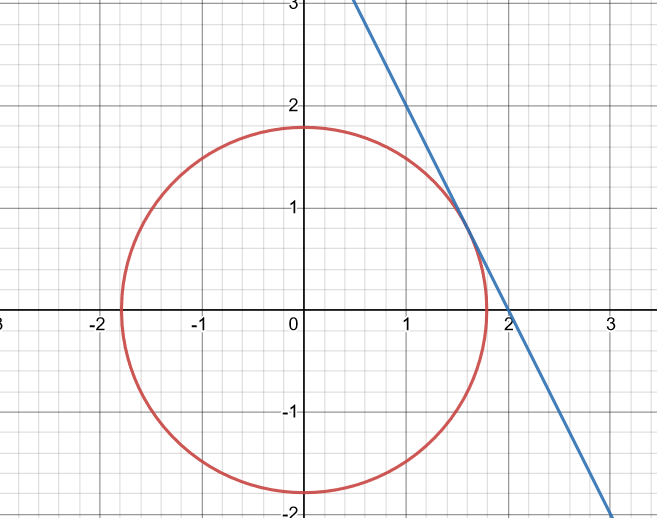
\includegraphics[scale=1.5]{image.png}
\vspace{5mm}

\section{Problem 10.3}
	Let $u \in \R^n$ be a vector such that for all $i \neq j$, $|u_i| \neq |u_j|$. We consider the constrained optimization problem
	$$
	\text{maximize} \quad \langle u ,x \rangle \quad \text{subject to} \quad \|x\|_1 \leq 1.
	$$

a) Calling $i_*$ the index at which $|u_i|$ is maximum, give a solution for the optimization problem (no Lagrange multiplier needed). \\
 
 Firstly, we need to understand that when we try to maximize the dot product of u and x, we are really trying to maximize the sum of the multiplication of their respective entries, that is to say, we want to maximize: $u_ix_i + \dots + u_nx_n$. Also, its important to note that we know that the sum of the absolute values of x are less than or equal to 1, that is to say: $|x|_1 \leq 1$ or $|x_1| + \dots + |x_n| \leq 1$. Lets pick the maximum entry of u, and call it $u_*$ which is at entry $u_{i*}$ Since we have the l1 norm constraint, lets define each $u_i$ as $|u_i| = |u_i| = |u_i*| - \beta_i$ where $\beta_i \geq 0$ Then we have:
 $$
    \langle u, x \rangle \leq |x_1|(|u_1|-\alpha_1) + \dots |x_n|(|u_n| - \alpha_n)
 $$
We can then manipulate the expression in the following way:
\begin{equation}
    \begin{split}
        \langle u, x \rangle &\leq |x_1||u_1| + \dots |x_n||u_n| \\
        \langle u, x \rangle &\leq  \sum_{i \neq i_*}^n |x_i|(|u_i|-\alpha_i) + (|u_*| - \alpha_{i*})|x_n| \\ 
        \langle u, x \rangle - \sum_{i \neq i_*}^n |x_i|\alpha_i &\leq |u_*|||x||_1
    \end{split}
\end{equation}

Therefore, the solution to this problem is a vector that contains all 0's except for the entry at the index that corresponds to the largest value of u ($u_{i*}$), which will be either $-1$ or $1$. We will call this solution $x_*$ This makes sense, as the largest value that an entry can take in x vector is either -1, or 1, due to the l1 norm constraint. Part c illustrates geometrically how this works, and provides great intuition for the solution.\\

b) By contradiction, show that this solution is unique.\\

We have found that the solution to our problem is when the vector $x$ is all 0's except for the entry corresponding to the maximum absolute value entry $u_{i*}$ in the vector (when $x_*=x_{i*}$). To prove that this is unique, lets assume that $x_* \neq x_{i*}$ and instead $x_* = x_j$. If $x_* = x_j$ then there is a scenario in which some $i\neq i*$ then some $x_i \neq 0$ (it would mean the other entries wouldn't have to be minimized). If this is the case, then we can look at our answer in part a and note that in the inequality each term before it is reduced by the corresponding term within our summation. Therefore, it cannot produce the maximum we found in part a, $x_*$ Therefore, we have shown that the solution in part a is unique, and that $x_*$ is maximized only when $x_* = x_{i*}$  \\

\newpage 

c) Give a graphical interpretation in the case $n=2$. You should consider the orthogonal projector onto $Span(u)$.\\

In this image, the red counter line is the l1 norm, the black line is the vector x such that it maximizes the dot product between x and u, and the blue vector is u. The green vector is the orthogonal projection of x onto the subspace spanned by u.

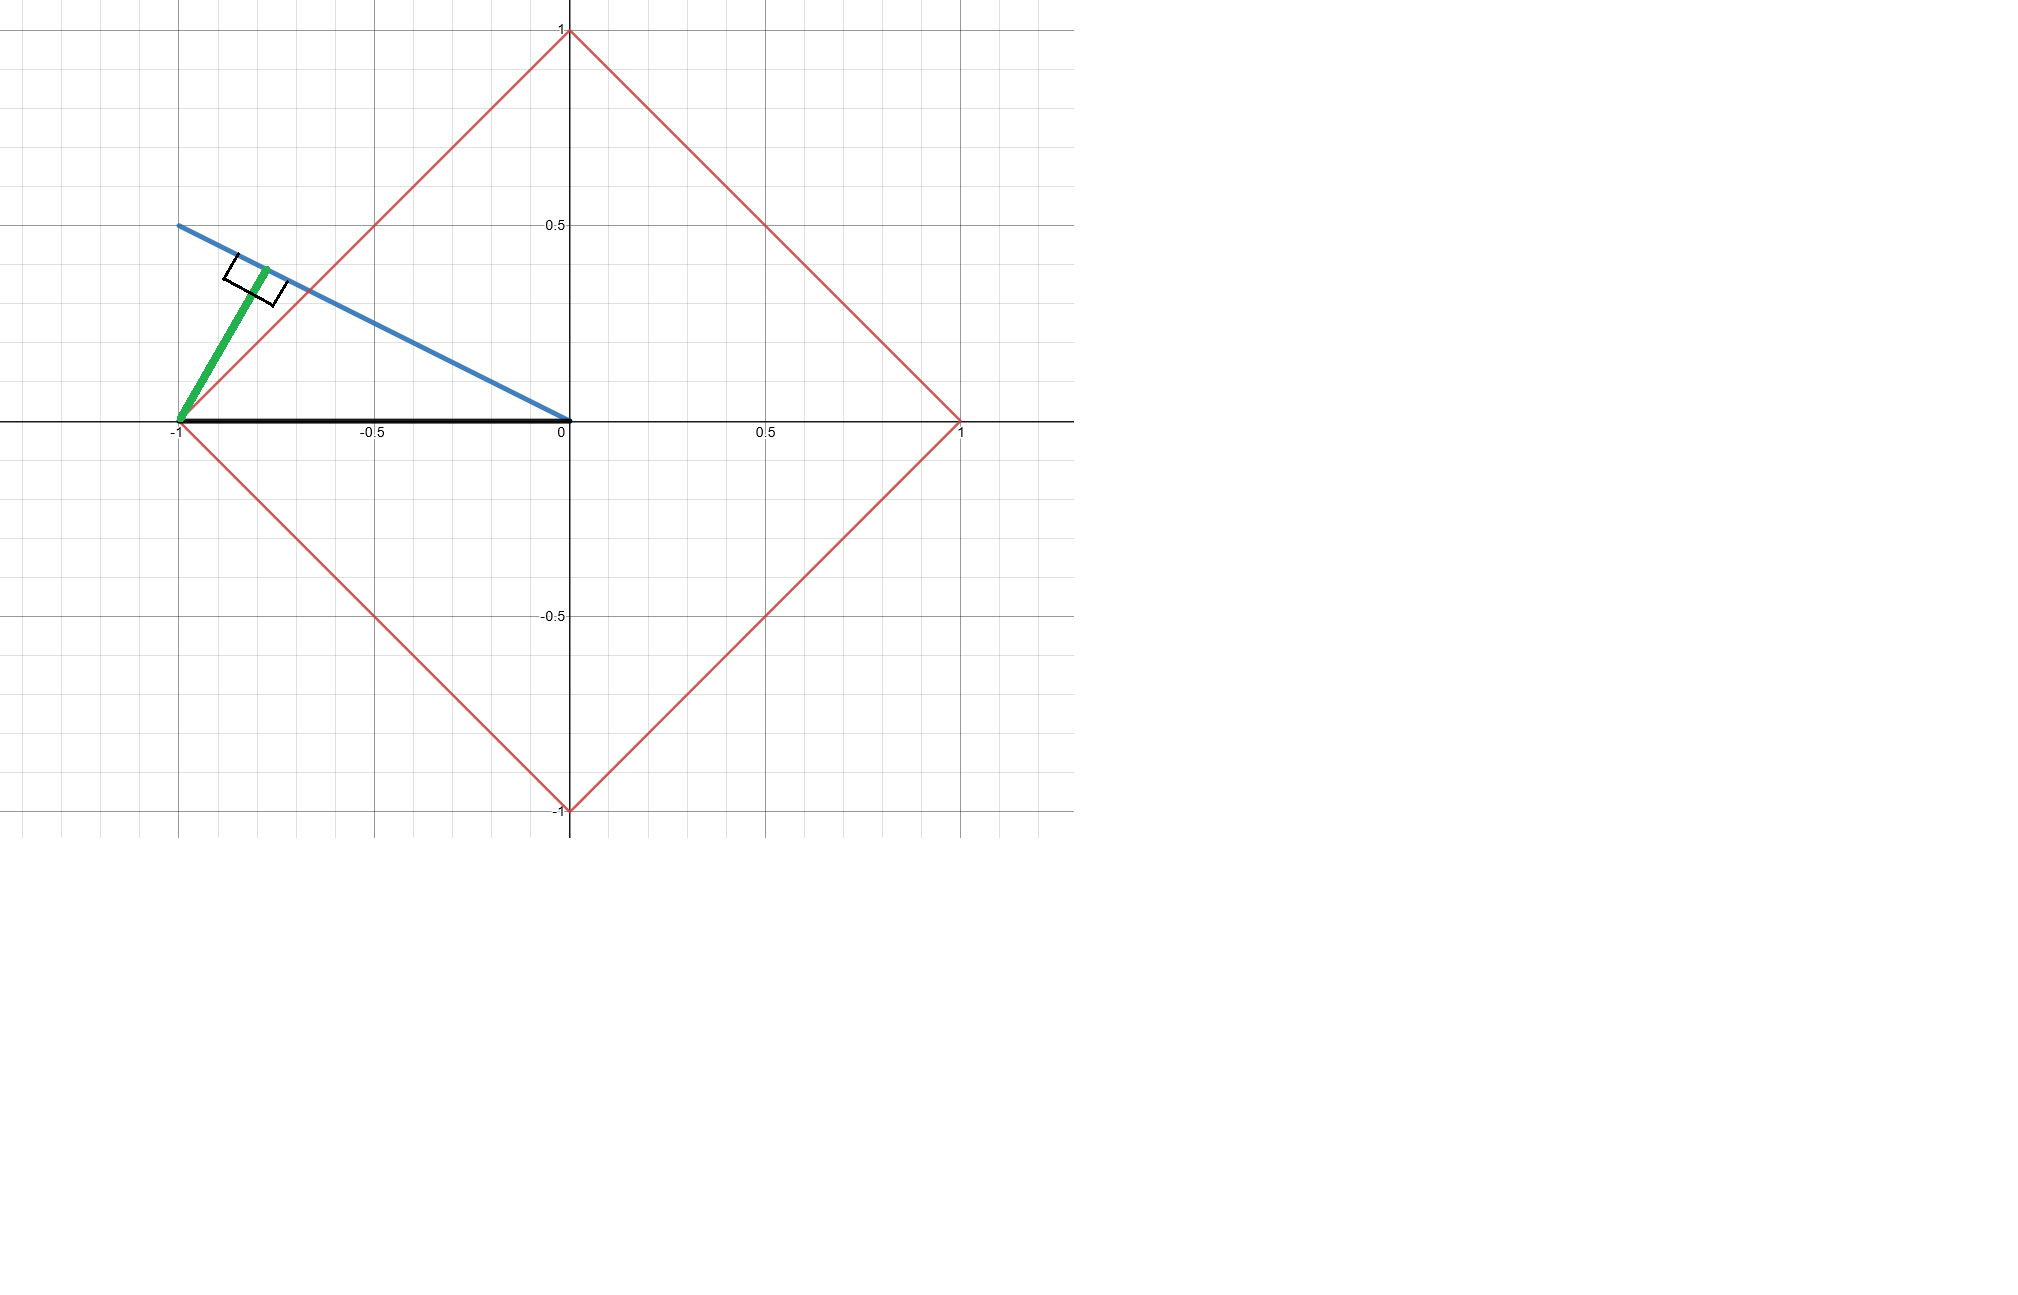
\includegraphics[scale=.5]{image2.png}



\newpage

\section{Problem 10.4}
	\emph{\textbf{We will prove the spectral theorem in this problem: you are therefore not allowed to use the spectral theorem and its consequences to solve this exercise.}}

	Let $A$ be an $n \times n$ symmetric matrix. We consider the following optimization problem
	\begin{equation}\label{eq:eig1}
		\text{maximize} \quad x^{\sT} A x \quad \text{subject to} \quad \|x\| = 1.
	\end{equation}
	This optimization problem admits a solution (this comes from the fact that a continuous function on a compact set achieved its maximum) that we denote by $v_1$.\\

a) Using Lagrange multipliers, show that $v_1$ is an eigenvector of $A$.\\
Lets set up our Lagrangian function by defining 
$$
g(x) = x^TAx \text{ and } h(x) = ||x|| = 1 \rightarrow x^Tx - 1 = 0$$
But wait! Since we want to maximize $x^TAx$, we can't use the normal procedure. We must first realize that maxizing $x^TAx$ is the same as minimizing $-x^TAx$, so $g(x) = -x^TAx$.
Then we have:
$$
    \Lagr (x,\lambda) = g(x) + \lambda h(x) = -x^TAx + x^Tx - 1
$$
We can now take the gradient of the function and analyze its critical points:
\begin{equation}
    \begin{split}
    \nabla (x, \lambda) &= \nabla g(x) + \nabla \lambda h(x)   \\
    \frac{\partial g}{\partial x} &= -2Ax \\
    \frac{\partial h}{\partial x} &= 2\lambda x \\
    \frac{\partial \Lagr}{\partial x} &= -2Ax + 2\lambda x 
    \end{split}
\end{equation}
Setting the gradient of the Lagrange to 0 we have:
\begin{equation}
    \begin{split}
        -2Ax + 2\lambda x &= 0 \\
        2Ax &= 2\lambda x \\
        Ax &= \lambda x
    \end{split}
\end{equation}
Which is the exact definition of a matrix transformation (A) acts on an eigenvector (x) with an eigenvalue ($\lambda$). Therefore, x is an eigenvector with associated eigenvalue $\lambda$.

\newpage

b) We now consider the optimization problem
	\begin{equation}
		\text{maximize} \quad x^{\sT} A x \quad \text{subject to} \quad \|x\| = 1
		\quad \text{and} \quad \langle x,v_1 \rangle = 0.
	\end{equation}
	For the same reason as above, this problem admits a solution that we denote by $v_2$. Show that $v_2$ is an eigenvector of $A$ that is orthogonal to $v_1$.\\
We will repeat the same procedure as we did in part a, but this time with two constraints. Lets define the following:
$$
    g(x) = x^TAx \ h(x) = x^Tx \ k(x) = x^Tv_1
$$
Then our Lagrangian function will be the following:
$$
    \Lagr (x,\lambda_1, \lambda_2) = g(x) + \lambda_1 k(x) + \lambda_2 h(x) 
$$
We now take the gradient of the Lagrangian and set it to 0.

\begin{equation}
    \begin{split}
    \nabla \Lagr (x, \lambda_1, \lambda_2) &= \nabla g(x) + \nabla \lambda_1 k(x)  + \nabla \lambda_2 h(x) \\
    \frac{\partial g}{\partial x} &= -2Ax \\
        \frac{\partial k}{\partial x} &= \lambda_1 v_1 \\
    \frac{\partial h}{\partial x} &= 2\lambda_2 x \\
    \frac{\partial \Lagr}{\partial x} &= -2Ax + \lambda_1 v_1 + 2\lambda _2x 
    \end{split}
\end{equation}

 We will have to manipulate the expressions using the constraints to tease out the solution:
 
\begin{equation}
    \begin{split}
        0 &= -2Ax + \lambda_1 v_1 + 2\lambda_2 x  \\
        0 &= -2v_1^TAx + \lambda_1 v_1^Tv_1 + 2\lambda_2 v_1^Tx \\
        0 &= -2v_1^TAx + \lambda_1 + 2 \times 0 \\
        \lambda_1 &= 2 \langle v_1, Ax \rangle \\
        \lambda_1 &= 2 \langle Ax, v_1 \rangle \\
        \lambda_1 &= 2 x^TA^Tv_1 \\ 
        \lambda_1 &= 2x^TAv_1\\
        \lambda_1  &= 2\lambda_1 x^Tv_1 \\  
        \lambda_1  &= 2\lambda_1 \times 0 \\
        \lambda_1 &= 0
    \end{split}
\end{equation}
We arrive at this solution by applying a few tricks. Firstly, we multiplied each side by $v_1^T$, then we used the fact that $\langle v_1, x \rangle = 0$ and $||v_1|| = 1$ to simplify. Then we used the fact that the dot product is a linear operation closed under addition, then that A is a symmetric matrix, and then that $v_1$ is an eigenvector of A. We find that $\lambda_1=0$, which we can plug back into our equation to find $\lambda_2$.

\begin{equation}
    \begin{split}
        0 &= -2Ax + \lambda_1 v_1 + 2\lambda_2 x  \\
        0 &= -2Ax + 2\lambda_2x \\
        Ax &= \lambda_2 x \qed
    \end{split}
\end{equation}

Which shows that x is another eigenvector of A, which is orthogonal to $v_1$ and has the associated eigenvalue $\lambda_2$.\\


c) We now consider the optimization problem
	\begin{equation}\label{eq:eig3}
		\text{maximize} \quad x^{\sT} A x \quad \text{subject to} \quad \|x\| = 1
		\quad \text{and} \quad \langle x,v_1 \rangle = 0
		\quad \text{and} \quad \langle x,v_2 \rangle = 0.
	\end{equation}
	Again, this problem admits a solution that we denote by $v_3$. Show that $v_3$ is an eigenvector of $A$ that is orthogonal to $v_1$ and $v_2$.

	\emph{
		\textbf{Conclusion}: by repeating this procedure, we obtain an orthonormal family $v_1, \dots, v_n$ of eigenvectors of $A$. This proves the spectral theorem (without using any linear algebra result!).
	}
	\\
	
We repeat the same procedure that we did in b, but now with 3 constraints. Lets call the following:
$$
    g(x) = x^TAx \ h(x) = x^Tx-1 \ k(x) = x^Tv_1 \ j(x) = x^Tv_2 
$$
We now take the Lagrange:
\begin{equation}
    \begin{split}
    \nabla \Lagr(x, v_1,v_2,\lambda_1, \lambda_2, \lambda_3) &= \nabla g(x) + \nabla \lambda_1 k(x)  + \nabla \lambda_2 j(x) + \nabla \lambda_3 h(x) \\
    \frac{\partial g}{\partial x} &= -2Ax \\
        \frac{\partial k}{\partial x} &= \lambda_1 v_1 \\
        \frac{\partial j}{\partial x} &= \lambda_2 v_2 \\
    \frac{\partial h}{\partial x} &= 2\lambda_3 x \\
    \frac{\partial \Lagr}{\partial x} &= -2Ax + \lambda_1 v_1 + \lambda_2 v_2 + 2\lambda_3x 
    \end{split}
\end{equation}

Now we set the gradient to 0 and solve for the lambdas:

\begin{equation}
    \begin{split}
        0 &= -2Ax + \lambda_1 v_1 + \lambda_2 v_2 + 2\lambda_3x  \\
        0 &= -2v_1^TAx + \lambda_1 v_1^Tv_1 + \lambda_2 v_1^Tv_2 + 2\lambda_3 v_1^Tx \\
        0 &= -2v_1^TAx + \lambda_1 \\
        \lambda_1 &= 0
    \end{split}
\end{equation}

And we have found that $\lambda_1 = 0$. I didn't write some of the intermediate steps, as they are just repeats of the procedure we defined in b, in which we can manipulate the expression such that the orthogonal vectors equal 0 via dot product. Now we repeated the process for $\lambda_2$

\begin{equation}
    \begin{split}
        0 &= -2Ax + \lambda_1 v_1 + \lambda_2 v_2 + 2\lambda_3x  \\
        0 &= -2v_2^TAx + \lambda_1 v_2^Tv_1 + \lambda_2 v_2^Tv_2 + 2\lambda_3 v_2^Tx \\
        0 &= -2v_2^TAx + \lambda_2 \\
        \lambda_2 &= 0
    \end{split}
\end{equation}

And using the same procedure we have found that $\lambda_2 = 0$. We can now plug in the values for the first two lambdas to find the final one.
\begin{equation}
    \begin{split}
        0 &= -2Ax + \lambda_1 v_1 + \lambda_2 v_2 + 2\lambda_3x  \\
        0 &= -2Ax + 2\lambda_3x \\ 
        Ax &= \lambda_3x \qed
    \end{split}
\end{equation}
And here we have shown that x is an eigenvector of A with associated eigenvalue $\lambda_3$ and is orthogonal to $v_1,v_2$.

\newpage 

\section{Problem 10.5}
	We consider the problem with physics motivation of finding the maximal entropy distribution of a random variable (see last slides of Lecture 09)  constraining values of some moments. \\
	

	To keep things simple, we consider $X$ that can take $n$ different values $x_1, \cdots, x_n$ in $\R$. We wish to infer the probabilities $p_1, \cdots, p_n$ such that the entropy is maximal and the expected value of $X$ is equal to a previously known scalar $\mu \in \R$. This corresponds to solving the contrained optimization problem
	\begin{equation}\label{eq:eig3}
		\text{maximize} \quad - \sum_i p_i \ln p_i \quad \text{subject to} \quad p_i \geq 0 \text{ for all } i
		\quad \text{and} \quad \sum_{i=1}^n p_i = 1
		\quad \text{and} \quad \sum_{i=1}^n p_i x_i = \mu.
	\end{equation}

a) Rewrite the problem as a convex minimization problem (justify). \\

We can note that maximizing $-\sum_i p_i \ln p_i$ is the same as minimizing $\sum_i p_i \ln p_i$. Given that, we can rewrite the problem statement such that it is a convex minimization problem:

$$
 Minimize \ \sum_i p_i \ln p_i \qquad \text{subject to: }
 p_i \geq 0 \text{ for all } i
		\quad \text{and} \quad \sum_{i=1}^n p_i = 1
		\quad \text{and} \quad \sum_{i=1}^n p_i x_i = \mu$$ 
		
We can do so with Lagrange minimization technique that we have used in the above problems. Firstly, lets pack our p and x values into vectors in $\R^n$ such that $p \in \R^n$ and $x \in \R^n$ where $p_i = p_i$ and $x_i = x_1$. Also, let $1$ refer to the a vector in $\R^n$ where all the entries are equal to 1. Also, let $l \in \R^n$ where $l_i = ln(p_i)$. Then lets note the following:

\begin{equation}
    \begin{split}
         &\sum_i p_i \ln p_i \rightarrow \langle p_i, l_i \rangle \qquad \\
         &\text{where } l \in \R^n \text{ and } l_i = ln(p_i) \\
         &\sum_{i=1}^n p_i = 1 \rightarrow \sum_{i=1}^n p_i - 1 = 0 \rightarrow \langle p_i, 1 \rangle -1 = 0 \\
         &\text{ where } 1 \text{ refers a vector in } \R^n \text{ with all of its values equal to 1}\\
         & \sum_{i=1}^n p_i x_i = \mu \rightarrow \sum_{i=1}^n p_i x_i - \mu = 0  \rightarrow \langle p_i, x_i \rangle -\mu = 0
    \end{split}
\end{equation}

We can then use the Lagrange function to find the solution to our constrained minimization problem (which will be the solution to the maximization problem in the problem statement as we flipped the sign of the original function). Our constrained optimization function now takes the form:
$$
    \Lagr (p,x,\mu, \lambda_1,\lambda_2) = \langle p_i, l_i \rangle + 
    \lambda_1(\langle p_i, 1 \rangle -1) + \lambda_2(\langle p_i, x_i \rangle -\mu)
$$

\newpage

b) Using KKT theorem, give the expression of the probability vector solution $p \in \R^n$ as a function of Lagrange multipliers and values $x_i$. Give also the relations between the Lagrange multipliers, $\mu$ and values $x_i$.\\
We can give the expression of the probability vector solutions as a function of the Lagrange multipliers by taking the gradient of the lagrange function and setting it equal to 0, then solving for the system of equations that results.
As we have: 
$$
    \Lagr (p,x,\mu, \lambda_1,\lambda_2) = \langle p_i, l_i \rangle + 
    \lambda_1(\langle p_i, 1 \rangle -1) + \lambda_2(\langle p_i, x_i \rangle -\mu)
$$
Then: 
\begin{equation}
    \begin{split}
        \nabla \Lagr (p,l,x,\mu, \lambda_1,\lambda_2) &=  \Lagr' (p,l,x,\mu, \lambda_1,\lambda_2)\\
        \frac{\partial \Lagr}{\partial p} &= l_i + \lambda_1 + \lambda_2 x_i \\
        \frac{\partial \Lagr}{\partial x} &= \lambda_2 p_i \\
        \frac{\partial \Lagr}{\partial \mu} &= 0 \\
        \frac{\partial \Lagr}{\partial \lambda_1} &= \langle p_i, 1 \rangle -1 \\
        \frac{\partial \Lagr}{\partial \lambda_2} &= \langle p_i, x_i \rangle -\mu
    \end{split}
\end{equation}
Setting the gradient equal to 0, we can see that:
$$-\frac{l_i+\lambda_1}{x_i} = \lambda_2 \text{ and that } \lambda_2 p_i = 0$$
. We can use this information to find the critical points of our function.  

\begin{equation}
    \begin{split}
        
    \end{split}
\end{equation}

\\
c) In the case where $n=2$ and $x_1=0$ and $x_2=1$, solve for the values of the Lagrange multipliers and $p \in \R^2$. Could you have used an easier way to solve the problem in this simple case?




\end{document}
